\subsection{Couches OSI}
\begin{table}[H]
\centering
\begin{tabular}{cm{2.2cm}l m{5cm} m{5cm}}
N & Nom & unité & description & exemples\\\hline\hline
7 & Application (\emph{Application}) & Donnée & Utilité pour l'utilisateur (transfert de fichiers, vidéos, etc...) & FTP, IMAP, HTTP\\\hline
6 & Présentation (\emph{Presentation}) & Donnée & Formats, mises en formes, cryptage, login & JSON, ASCII, HTML, Unicode\\\hline
5 & Session (\emph{Session}) & Donnée & Gestion de l'activité & RPC, NetBios\\\hline
4 & Transport (\emph{Transport}) & Segment, Datagramme & sous-adressage, communication entre deux processus & notion de port (TCP, UDP)\\\hline
3 & Réseau (\emph{Network}) & Paquet & Addressage logique (IP addr.) & IPv4/IPv6\\\hline
2 & Liaison (\emph{Data Link}) & Trame & Adressage physique (MAC addr.) & Ethernet, CAN \\\hline
1 & Physique (\emph{Physical}) & Bit, Symbol & Signaux électriques & Filaire ou sans-fil
\end{tabular}
\end{table}
Les couches 1-3 sont les couches matérielles. Les couches 4-7 sont les couches hautes liées à l'utilisation faite des données.

\begin{figure}[H]
    \centering
    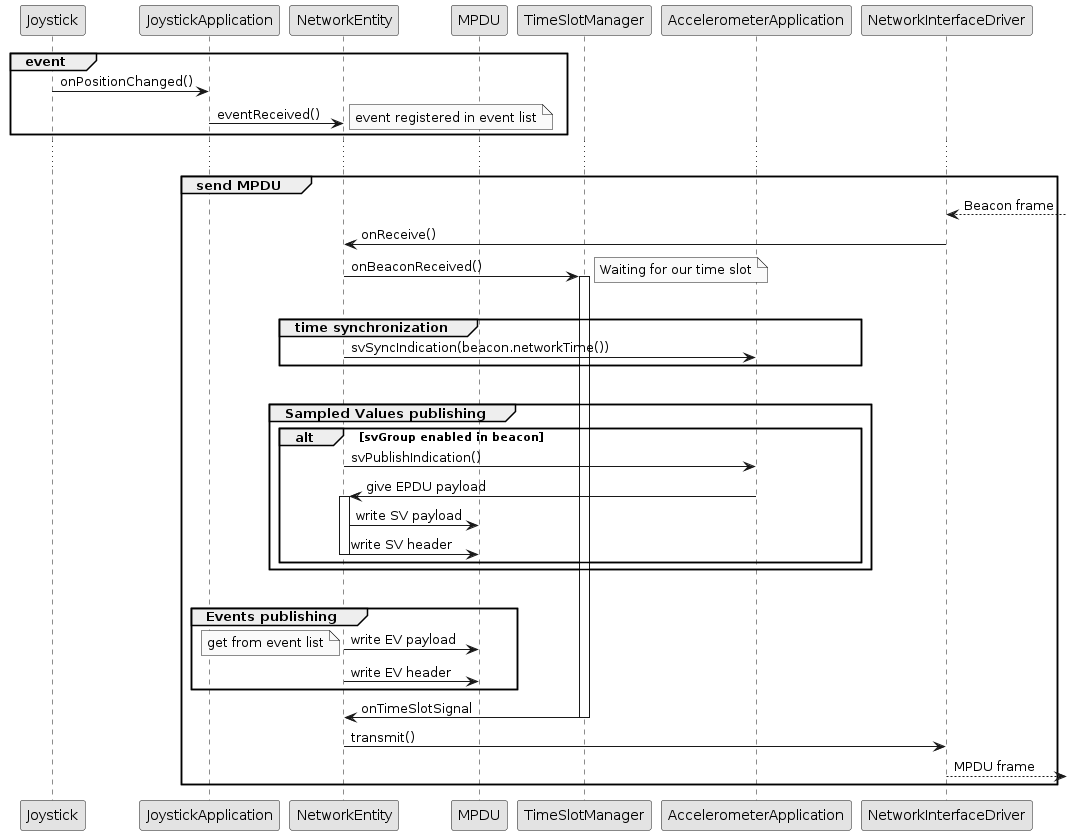
\includegraphics[width=0.9\linewidth]{figures/DeSEnet_sequence.png}
\end{figure}